\chapter{Introduzione}

\section{Electrical Mobility}

Al giorno d'oggi l'Electrical Mobility (EM) è considerata una degli elementi chiave per ridurre l'inquinamento 
e affrancarsi dalla dipendenza dai combustibili fossili. Questo sta inducendo governi e industrie automobilistiche a investire somme ingenti nei relativi progetti. 
\\\\
Si prevede che nel breve periodo il mercato legato all'EM sia destinato a crescere rapidamente come conseguenza dell'incremento della varietà di Veicoli Elettrici (EV) immessi sul mercato dalle Case Automobilistice. Secondo recenti studi infatti il numero di EV venduti nel periodo tra il 2010 e il 2012 è aumentato del 200\%. 
\\\\
Nonostante il crescente interesse nei confronti dell'EM, recenti analisi di mercato dimostrano che i benefici ad essa legati diverranno significativi soltanto nel lungo periodo, tesi confermata da una ricerca condotta dal U.S. National Energy Technology (\cite{katmale2011}) secondo la quale il 70\% dei potenziali consumatori non acquisterà un EV a causa dell'incertezza sulla disponibilità delle stazioni di ricarica. A questo si aggiungono le note problematiche riguardanti la capacità e la durata delle batterie nonché i significativi tempi di ricarica eccessivamente lunghi (nell'ordine delle decine di minuti) se comparati con quelli di rifornimento dei veicoli a combustibile fossile.
\\
Da un lato la durata dei tempi di ricarica, la limitata capacità delle batterie e la disposizione territoriale degli Electric Vehicle Supply Element (colonnine di ricarica - EVSE) influisce direttamente sull'esperienza di guida di ogni autista e può avere un impatto decisivo sulla penetrazione di mercato dei veicoli elettrici. D'altro canto diversi studi hanno dimostrato che l'impatto critico sulla rete energetica causato dalla ricarica simultanea di un numero significativo di EV. Si è quindi delineata chiaramente la necessità di coordinare efficacemente le necessita di ricarica degli EV con la quantità e la dislocazione territoriale degli EVSE.
\\\\
Molti progetti Europei sono stati avviati con lo scopo di limitare queste problematiche. Allo stesso tempo bisogna considerare che un uno scenario realistico di EM coinvolge diverse parti interessate (autisti, case automobilistiche, produttori di energia, traffico cittadino, fattori economici e psicologici ecc\dots). Uno scenario cosi complesso ha mobilitato la ricerca in direzione dell'Information and Communication Technology (ICT) per fornire servizi di supporto all'EM consentendo alle parti interessate di cooperare in modo intelligente e sostenibile.
Sono state sviluppate finora diverse applicazioni relative a scenari in scala ridotta ma si è ancora lontani dall'ottenere una effettiva interoperabilità tra gli attori in gioco sopratutto per la mancanza di standardizzazione delle tecnologie e dei dispositivi utilizzati.
\\\\
Stante l'elevato costo dei test su larga scala, la simulazione rappresenta lo strumento più adatto a testare l'efficacia delle soluzioni ICT prima che vengano realmente implementate (\cite{felice2012group}). A tutt'oggi sono stati sviluppati sia alcuni simulatori veicolari che permettono un controllo molto fine a livello di singolo veicolo che modelli di batteria atti a simulare realisticamente le dinamiche di carica e scarica. Tuttavia nessuno di questo strumenti è risultato efficace nella soluzione delle complesse dinamiche derivanti dall'impatto degli EV sulla rete elettrica cittadina e dalle incertezze sull'effettiva utilità dell'uso di sistemi di prenotazione delle ricariche. 
\\\\
Il progetto Internet of Energy (IoE) for Electrical Mobility, avviato dall'Unione Europea e comprendente 40 partner da 10 nazioni Europee, intende colmare queste lacuna tramite lo sviluppando di hardware, software e sistemi middleware che possano fornire un infrastruttura di comunicazione interoperabile tra le parti in gioco all'interno della cosiddetta grid ovvero il sistema formato dall'insieme delle stazioni di ricarica dislocate strategicamente sul territorio, dalle modalità di prenotazione programmata delle ricariche, dai dispositivi hardware atti a gestirle e dal software di controllo dell'intero sistema.
\\\\
Lo scopo di questa tesi, frutto del lavoro congiunto tra UNIBO e ARCES, seguito della tesi di laurea di Federico Montori, è quello di fornire un contributo significativo in questa direzione.

\section{Internet of Energy}

Internet of Energy è un progetto del framework ARTEMIS che da tre anni si concentra sullo sviluppo di tecnologie atte a realizzare e supportare l'adozione su larga scala della EM in Europa. Riunisce 40 partner di 10 paesi europei con l'obiettivo di mobilitare le migliori capacità industriali e di ricerca nei settori di produzione e stoccaggio dell'energia, sistemi embedded e produzione di veicoli elettrici. Il budget totale del progetto IoE è di 45 milioni di Euro, di cui la metà finanziata da 40 industrie partner.

Gli elementi fondamentali del progetto sono:

\begin{itemize}
	\item La cosiddetta \emph{smart-grid} (\cite{bedogni2013machine}) ovvero, in sintesi, la connessione delle reti energetiche ad Internet per consentire il controllo intelligente dell'energia prodotta da fonti rinnovabili, il suo stoccaggio e la sua distribuzione.
	\item La progettazione di veicoli elettrici che, mediante apposite tecnologie e dispositivi hardware e software, aumentino il rendimento dei motori elettrici minimizzando al contempo il consumo dell'energia immagazzinata nelle batterie.
	\item L'utilizzo di Internet per l'interconnessione tra la smart-grid, i veicoli elettrici e gli utenti al fine di ottimizzare le operazioni di ricarica delle batterie compatibilmente con i vincoli imposti dal traffico cittadino e dal rapporto tra consumo e disponibilità globali di energia. In questo ambito si inserisce il progetto all'origine di questa tesi.
	\item La definizione di standard volti ad assicurare l'interoperabilità tra gli attori in gioco.
\end{itemize}

\begin{figure}[H]
	\centering
	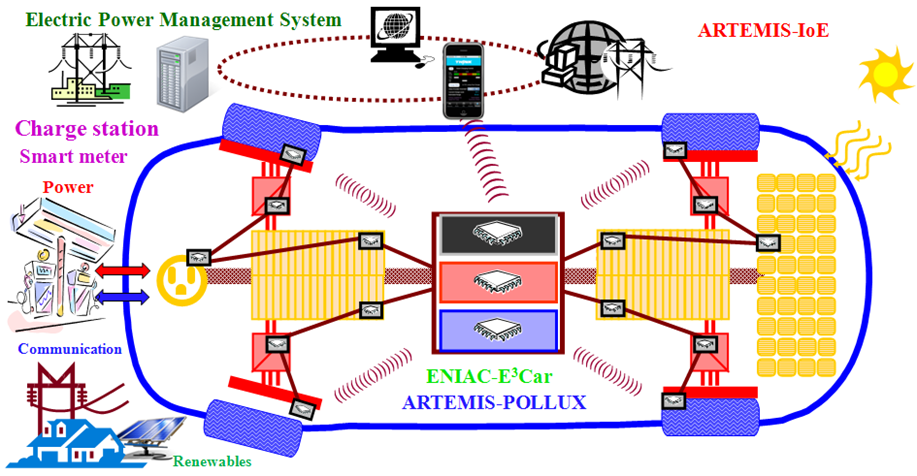
\includegraphics[width=1.0\textwidth]{assets/ioe.png}
	\caption{Overview del progetto Internet of Energy}
	\label{fig:ioe}
\end{figure}

\section{Contributo al progetto IoE}

L'Università di Bologna, congiuntamente ad ARCES, si propone di sviluppare una piattaforma software con l'obbiettivo di fornire una prima valutazione della compatibilità delle specifiche del progetto IoE con la realtà dello scenario cittadino Bolognese (\cite{bedogni2013interoperable}).

Innanzitutto è stato sviluppata un architettura software volta a fornire i servizi per l'interazione tra gli utenti e la smart-grid mediante tecnologie mobile. La connessione tra l'utente e la smart-grid è assicurata dal City Service (CS) a cui giungono le richieste di prenotazione di ricarica provenienti dagli smartphone, fornendo la lista delle colonnine disponibili che meglio si adattano alle esigenze dell'utente. I dati sono rappresentati mediante un grafo semantico e la loro definizione avviene tramite ontologia. Questo permette ai vari attori in gioco, di natura estremamente eterogenea, di comunicare e processare i dati in modo completamente trasparente. Attraverso l'ontologia vengono definite tutte le informazioni inerenti la smart-grid. La persistenza e la condivisione delle informazioni è assicurata da un repository semantico, il Semantic Information Broker (SIB), parte del progetto Smart-M3 (\cite{smart2013}). 

In secondo luogo è stata creata un'applicazione mobile che permette all'utente di monitorare i parametri della batteria del veicolo e di prenotare slot di tempo presso gli EVSE grazie all'interazione con il CS mediante un SIB dedicato. Il servizio di prenotazione da la possibilità all'utente di trovare l'opzione di ricarica più consona alle sue esigenze.

Infine è stata creata una piattaforma di simulazione integrata che permette di valutare su larga scala
l'impatto dell'introduzione della mobilità elettrica veicolare nel contesto urbano bolognese. Diversamente da altri tool esistenti il framework proposto permette di studiare il comportamento degli EV, con relativo modello di carica e scarica della batteria unitamente all'interazione di essi con la samrt-grid. 


%\section{Stato dell'Arte}



\section{Un po di storia}\label{sec:unpodistoria}

L'applicazione mobile è stato il mezzo che mi ha permesso di avere il privilegio di partecipare a questo progetto. Era il 19/07/2012 quando ho inviato al Prof \emph{Luciano Bononi} la richiesta di progetto per il corso di \emph{Laboratorio di Applicazioni Mobili}. Non potevo immaginare che quella email mi avrebbe portato ad un lavoro durato oltre un anno e che dura tutt'ora.
Al colloquio per l'assegnazione del progetto mi venne presentato l'opportunità di rendere più accattivante l'applicazione mobile creata da Federico Montori per il suo progetto di laurea. Questo perché, visto il poco tempo che egli aveva potuto dedicarci, era ancora in fase embrionale.
Cosi, in seguito a qualche meeting, con i vari componenti del progetto e notevoli dosi di pazienza da parte di \emph{Federico Montori}, che mi ha introdotto al progetto, sono riuscito a disporre un ambiente più o meno funzionate. La simulazione \emph{crashava} dopo un secondo ma tanto bastava per introdurre un veicolo ed eseguire i test con la nuova applicazione mobile.
Successivamente, capendo la vastità del progetto che stava dietro all'applicazione, decisi di farlo diventare progetto di laurea poiché era evidente che c'era ancora molto lavoro da fare e la mia innata capacità di complicarmi la vita ha giocato un ruolo fondamentale in tutto questo. Nel resto di questa tesi verrà spiegato come si è evoluta questa storia.
